\documentclass{report}
\usepackage[T1]{fontenc} % Fontes T1
\usepackage[utf8]{inputenc} % Input UTF8
\usepackage[backend=biber, style=ieee]{biblatex} % para usar bibliografia
\usepackage{csquotes}
\usepackage[portuguese]{babel} %Usar língua portuguesa
\usepackage{blindtext} % Gerar texto automaticamente
\usepackage[printonlyused]{acronym}
\usepackage{hyperref} % para autoref
\usepackage{graphicx}
\usepackage{titlesec}
\usepackage{float}

\bibliography{bibliografia}


\begin{document}
%%
% Definições
%
\def\titulo{Projeto 2: Biblioteca de imagens}
\def\data{08/05/2019}
\def\autores{André Patacas, Gil Teixeira, Sofia Vaz}
\def\autorescontactos{(93357) andrepatacas@ua.pt, (88194) gilteixeira@ua.pt, (92968) sofiateixeiravaz@ua.pt}
\def\versao{1}
\def\departamento{DETI}
\def\empresa{LABI}
\def\logotipo{ua.pdf}

%
%%%%%% CAPA %%%%%%
%
\begin{titlepage}

\begin{center}
\centering
%
\vspace*{50mm}
%
{\Huge \titulo}\\ 
%
\vspace{10mm}
%
{\Large \empresa}\\
%
\vspace{10mm}
%
{\large \autores}\\ 
%
\vspace{30mm}
%
\begin{figure}[h]
\centering
\includegraphics{\logotipo}
\end{figure}
%
\vspace{30mm}
\end{center}
%
\begin{flushright}
\versao
\end{flushright}
\end{titlepage}

%%  Página de Título %%
\title{%
{\Huge\textbf{\titulo}}\\
{\Large \departamento\\ \empresa}
}
%
\author{%
    \autores 
}
%
\date{\data}
%
\maketitle


\pagenumbering{roman}

%%%%%% RESUMO %%%%%%
\begin{abstract}
Este relatório pretende descrever como uma biblioteca de imagens pesquisável foi desenvolvida no âmbito da cadeira de Laboratório de Informática. Esta biblioteca de imagens foi feita com base em Python 3, \ac{CSS}, JavaScript e \ac{HTML}. Neste relatório incluímos a divisão geral do trabalho, a explicação geral de métodos criados no \textit{backend} e \textit{frontend} e imagens dos resultados. 
\end{abstract}

%%%%%% Agradecimentos %%%%%%
% Segundo glisc deveria aparecer após conclusão...

\tableofcontents
 \listoftables     % descomentar se necessário
 \listoffigures    % descomentar se necessário


%%%%%%%%%%%%%%%%%%%%%%%%%%%%%%%
\clearpage
\pagenumbering{arabic}

%%%%%%%%%%%%%%%%%%%%%%%%%%%%%%%%
\chapter{Introdução}
\label{chap.introducao}

O frontend da aplicação foi feito em \ac{HTML}, \ac{CSS} e JavaScript e o
backend foi feito em Python 3. A base de dados usada foi SQLite3. Esta aplicação 
foi feita no âmbito de Laboratórios de Informática no ano letivo 2018/2019.
A adicionar às especificações básicas pedidas no o guião sobre regras do segundo projeto, 
construiu-se ainda suporte para para pydocs e um sistema de pesquisa de imagens por qualquer 
cor do espectro rgb.
Este documento está dividido em quatro capítulos.
Depois desta introdução,
no \autoref{chap.metodologia} é apresentada a metodologia seguida, tendo em conta o trabalho faseado de cada um, 
no \autoref{chap.resultados} são apresentados os resultados obtidos,
sendo estes discutidos no \autoref{chap.analise}.
Finalmente, no \autoref{chap.conclusao} são apresentadas
as conclusões do trabalho.

\chapter{Metodologia}
\label{chap.metodologia}
\section{Definição de tarefas}
Esta fase consistiu em, antes de começar a trabalhar, definir quais membros do grupo fariam o quê, o que pode ser consultado na tabela \ref{tab:table1}: 
\begin{table}[h!]
\begin{center}
\caption{Divisão geral de tarefas}
\begin{tabular}{l|l}
\hline
\multicolumn{1}{|l|}{Aluno} & \multicolumn{1}{l|}{Tarefa Atribuída} \\ \hline
            André Patacas   & backend                               \\ 
            Gil Teixeira      & frontend                               \\
            Sofia Vaz         & relatório                                
\end{tabular}
\label{tab:table1}
\end{center}
\end{table}

\section{Backend}
Lista de fontes usadas nesta parte do projeto:
\begin{itemize}
\item \cite[\textit{Guião prático sobre CherryPy}]{guiãoCherryPy}
\item \cite[\textit{Guião prático sobre Bases de Dados}]{guiãoDB}
\item \cite[\textit{Guião prático sobre tratamento de imagem}]{guiãoIm}
\item \cite[\textit{Guião prático sobre aplicações móveis}]{guiãoMobi}
\item \cite[\textit{StackOverflow}]{SOvf}
\item \cite[\textit{Documentação relativa a CherryPy}]{CherryPy}
\end{itemize}
\subsection{DbCommunicator.py}
\paragraph{\_\_init\_\_}
Este método inicializa o objeto que comunica com a base de dados.

\paragraph{get\_dims\_and\_color}
Este método devolve os dados da imagem, a HUE da cor média e as dimensões. 

\paragraph{request\_caracteristics}
Este método liga-se ao \textit{website} fornecido pelos docentes, devolvendo um array em que cada elemento é um \ac{json} com:
\begin{itemize}
\item nome,  que é o resultado do \textit{hashing} do conteúdo das imagens para evitar imagens replicadas
\item classe
\item \textit{bounding box}, ou seja, a área onde a classe se verifica
\item "confiança" com a qual o servidor conseguiu classificar a imagem
\end{itemize}

\paragraph{add}
Este método adiciona uma imagem à base de dados. Se uma imagem tiver várias classes será cortada, 
tendo cada parte uma classe diferente, sendo também guardada a original. A base de dados terá a 
seguinte informação para cada objeto:
\begin{itemize}
\item nome
\item altura
\item largura
\item quantidade média de vermelho
\item quantidade média de verde
\item quantidade média de azul
\item \textit{boundig box}
\item confiança, de 0 a 1, de que a imagem foi classificada corretamente
\end{itemize}

\paragraph{remove}
Ao executar este método, uma dada imagem e todas as suas associadas serão removidas da base de dados.

\paragraph{get}
Este método devolve informação sobre uma imagem indentificada pelo id fornecido como parâmetro.

\paragraph{request}

Devolve uma string com os dados pedidos no argumento. O funcionamento é analogo ao descrito no enunciado.


\paragraph{Setup}
Ambos os métodos \_\_clear\_all\_caution\_\_ e  populate são usados para efeitos de \textit{setup} inicial.

\subsection{app.py}
Este programa serve os conteúdos estáticos \ac{HTML}, JavaScript e \ac{CSS} e cria uma API transformando os GET e POST requests em chamadas de funções comunicantes com a base de dados. 

\subsection{put\_example}
Este programa envia uma imagem para a base de dados, não tendo qualquer efeito na maneira como o \textit{website} funciona.

\section{Frontend}
Para uma biblioteca de imagens ser viável, a compatibilidade entre dispositivos é necessária. Por isso, na criação desta, foi sempre tida em conta a usabilidade não só em monitores de computador, mas também em dispositivos móveis. 
Lista de fontes usadas nesta parte do projeto:
\begin{itemize}
\item \cite[\textit{W3 Schools}]{W3}
\item \cite[\textit{StackOverflow}]{SOvf}
\item \cite[\textit{Documentação de JavaScript}]{JS}
\item \cite[\textit{Primeira fonte de imagens}]{Im1}
\item \cite[\textit{Segunda fonte de imagens}]{Im2}
\end{itemize}

\subsection{Home/Class List}
Esta página informa o utilizador de todas as classes já detetadas nesta biblioteca, mostrando alguns exemplos. Ao carregar no nome de uma classe, entra-se numa página em que todas as imagens da classe estão visíveis. Ao carregar numa imagem, o utilizador abre-a, vendo a imagem original e ainda as \textit{bounding boxes} de cada classe presente. O ficheiro \ac{JS} associado é class\_list.js.

\subsection{List Images}
Esta página mostra as imagens cortadas presentes na biblioteca sem nenhuma ordem em particular. Ao fazer \textit{hover} com o rato, é dada a informação sobre a classe detetada e a confiança com que foi classificada. Ao carregar no botão \textit{more}, é aberta a imagem numa nova pagina. Pode consultar o código desta página no ficheiro list\_images.html. O ficheiro \ac{JS} associado é image\_loader.js.


\subsection{Send Image}
Dá a possibilidade ao utilizador de inserir as próprias imagens na biblioteca. Para adicionar estes dados, o utilizador pode abrir o explorador de ficheiros a partir do botão da página ou arrastar uma para o \textit{form}. Se uma classe for detetada, então a base de dados será atualizada com a informação da nova imagem e esta ficará acessível a todos os utilizadores da biblioteca. O ficheiro \ac{JS} associado é send\_image.js.

\subsection{Inspect Image}
Esta página mostra a imagem  com as \textit{bounding boxes} de cada classe, informando o utilizador o que cada caixa é. O ficheiro \ac{JS} associado é image\_inspect.js.

\subsection{Search Images}
Esta página apresenta o motor de busca da biblioteca. É possível pesquisar por classe e por cor. 
A pesquisa por classe é feita a partir de uma caixa de texto em que são introduzidos dados e a pesquisa por cor é feita a partir de um seletor de cor, tornando a experiência o mais intuitiva possível para o utilizador. Para além disso, é possível definir a confiança mínima na deteção da classe e cor. Os ficheiros de \ac{JS} associados são handlers.js e image\_loader.js.

\subsection{About}
Aqui é possível encontrar os dados de todos os membros do grupo(nome, número mecanográfico, e-mail institucional) e a percentagem do trabalho feito por cada um.

\subsection{Pagina de Erro}
Esta página é mostrada quando ocorre um erro, desde tentativa de acesso a paginas que nao existem até erros internos.
Uma maneira de invocar um erro deste tipo é tentar aceder a imagens ou páginas que não existem. 


\subsection{Ficheiros .js}
\paragraph{class\_list}  Lista as classes já detetadas e apresenta imagens com exemplos.
\paragraph{handlers} Transforma os dados inseridos pelo utilizador sejam convertidos em dados utilizáveis pelos outros ficheiros de \ac{js}
\paragraph{class\_list}  Lista as classes já detetadas e apresenta imagens com exemplos.
\paragraph{image\_loader}Mostra as imagens segundo os dados inseridos pelo utilizador. 
Pesquisará segundo a classe se dados forem inseridos dados na caixa de texto. 
Se a caixa de \textit{Class Detection Confidence} estiver \textit{ticked}, então 
apenas serão mostradas imagens com uma confiança igual ou superior à selecionada. 
Se a caixa \textit{Search with color} estiver ativa, então as imagens surgirão segundo a 
sua proximidade com a cor selecionada. A caixa \textit{Color Confidence} tem funcionamento 
parecido com a \textit{Class Detection Confidence}. 
\paragraph{send\_image} Envia a imagem via POST request para o \textit{backend} do \textit{website}.
\paragraph{image\_inspect} Quando uma imagem é aberta, esta função mostra ao utilizador as \textit{bounding boxes} de cada classe e informação sobre estas. 


\chapter{Resultados}
\label{chap.resultados}
Nas imagens \ref{Fig1} e \ref{Fig2} é possível ver a página Class List, onde as classes detetadas até agora são listadas com alguns exemplos. 

\begin{figure}[H]
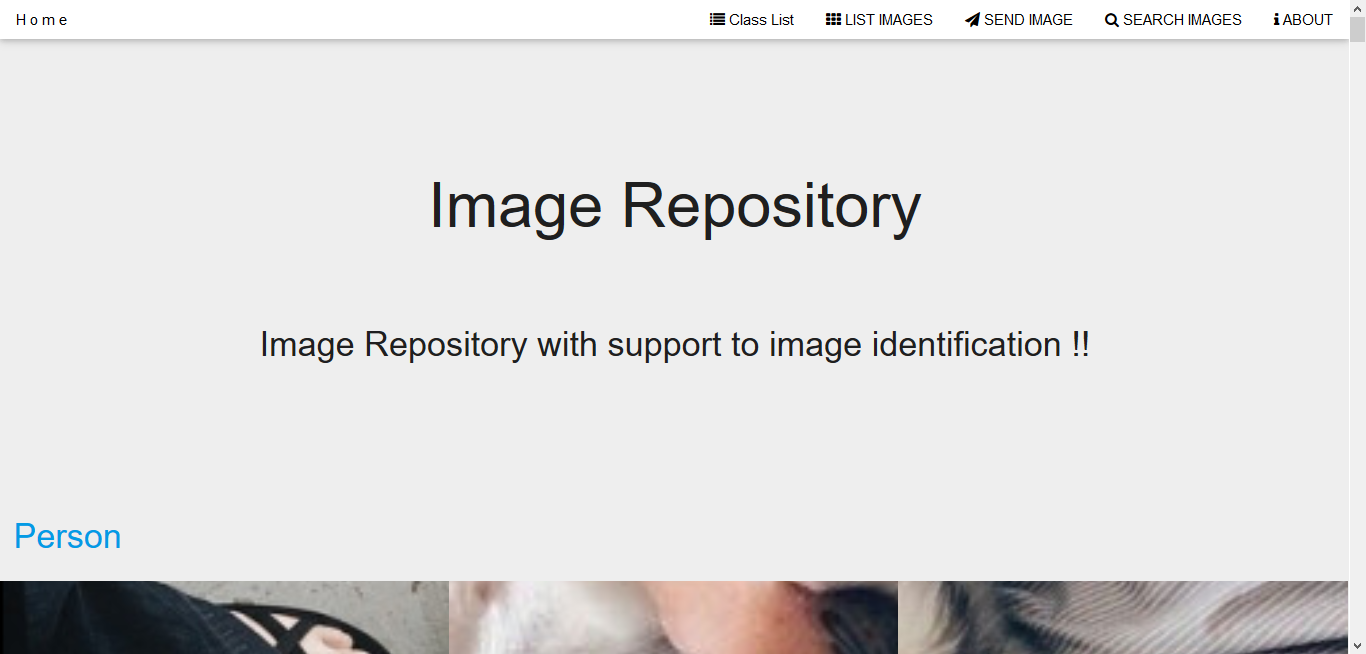
\includegraphics[width=\textwidth]{HomeTOP.png}
\caption{Topo da página Home/Class List}
\label{Fig1}
\end{figure}

\begin{figure}[H]
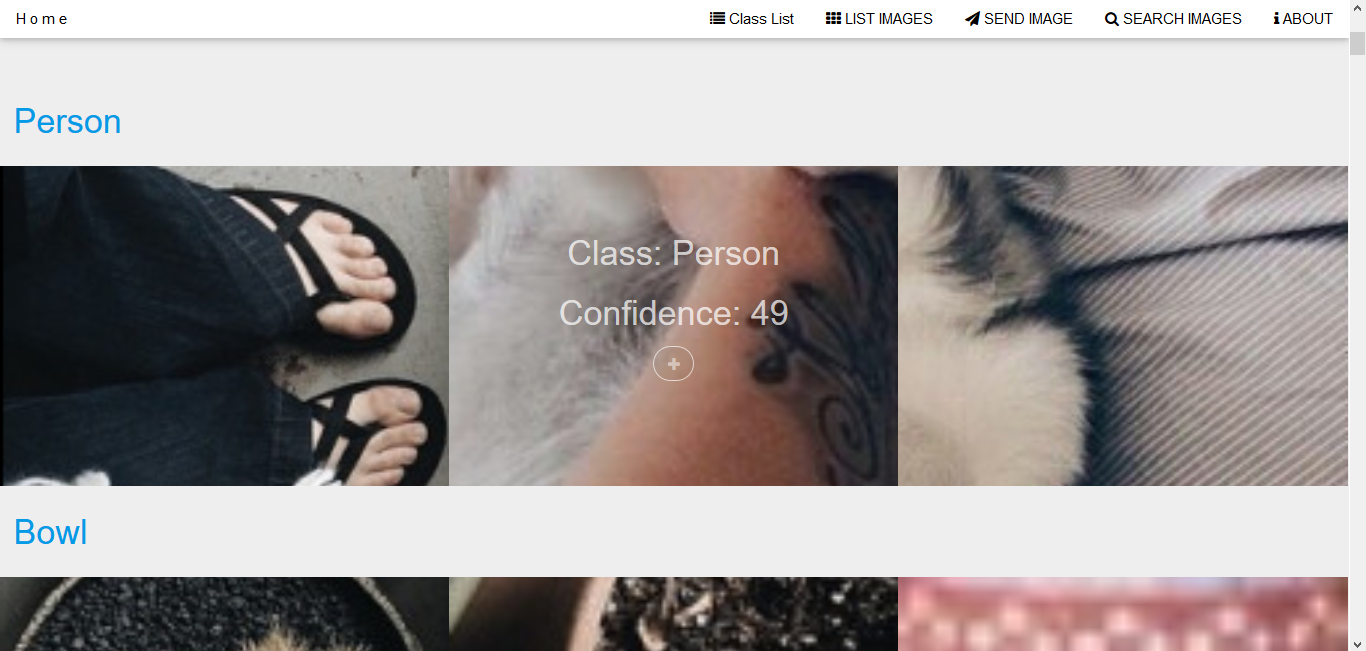
\includegraphics[width=\textwidth]{HomeBOTTOM.png}
\caption{Página Home/Class List com as imagens e classes visíveis}
\label{Fig2}
\end{figure}

Na imagem \ref{Fig3} é possível ver uma imagem aberta com as \textit{bounding boxes} (a azul) e a classe de cada \textit{bounding box} (a vermelho).

\begin{figure}[H]
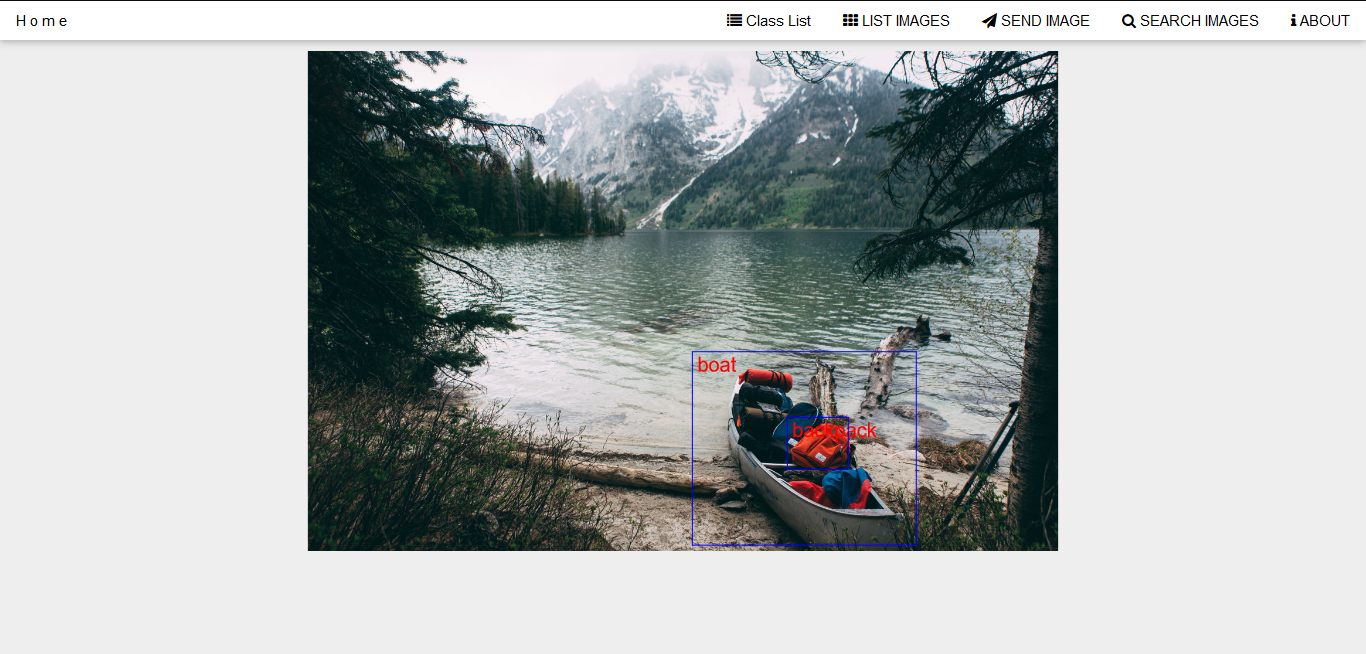
\includegraphics[width=\textwidth]{dataImage.png}
\caption{Dados de uma imagem aberta}
\label{Fig3}
\end{figure}

Na imagem \ref{Fig4} é possível ver os dados que uma imagem mostra quando é feito \textit{hover} com o rato, sendo estes dados a classe da imagem e a confiança.

\begin{figure}[H]
\includegraphics[width=\textwidth]{ExemploHOVER.png}
\caption{Efeito \textit{hover} numa imagem}
\label{Fig4}
\end{figure}

 Na imagem \ref{Fig5} vê-se a página List Images, sendo esta a página que lista todas as imagens sem nenhum critério de organização.

\begin{figure}[H]
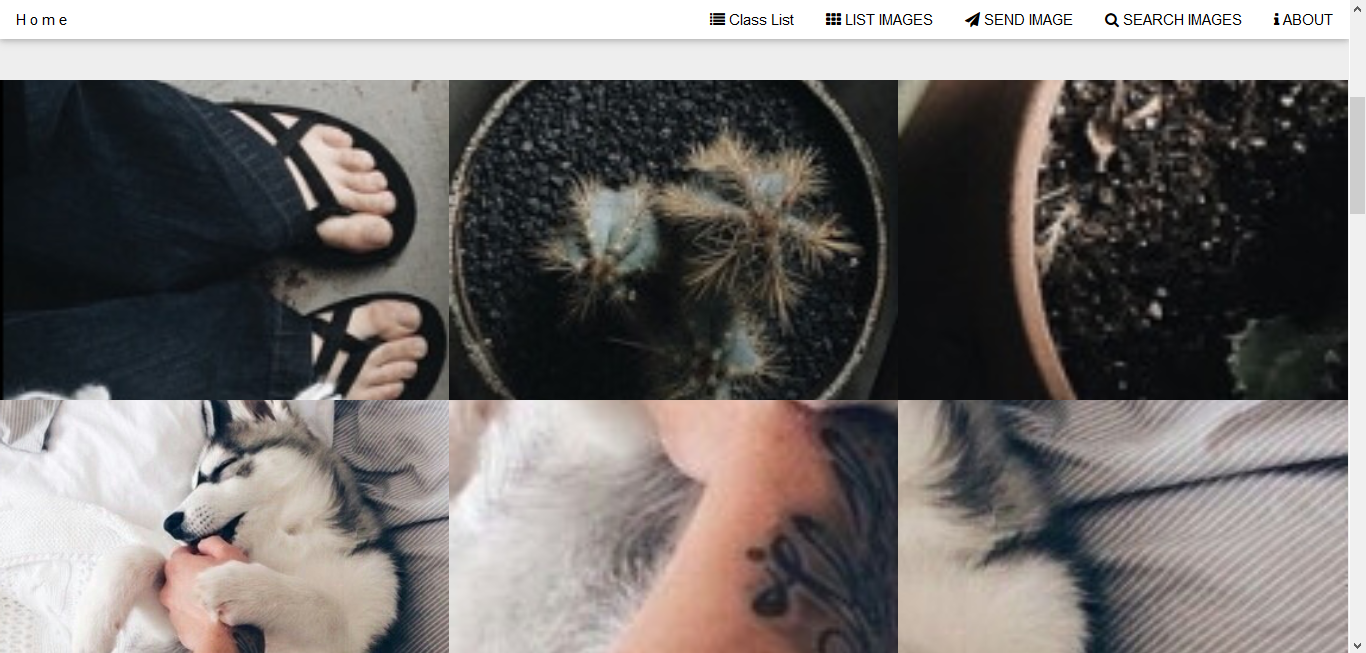
\includegraphics[width=\textwidth]{ListImages.png}
\caption{Página em que todas as imagens estão listadas}
\label{Fig5}
\end{figure}

Nas imagens \ref{Fig6}, \ref{Fig7} e \ref{Fig8} vê-se a página de pesquisa. Na primeira imagem a pesquisa não tem dados inseridos e na segunda procura-se por uma cor específica. Na terceira procura-se uma classe específica (cão).

\begin{figure}[H]
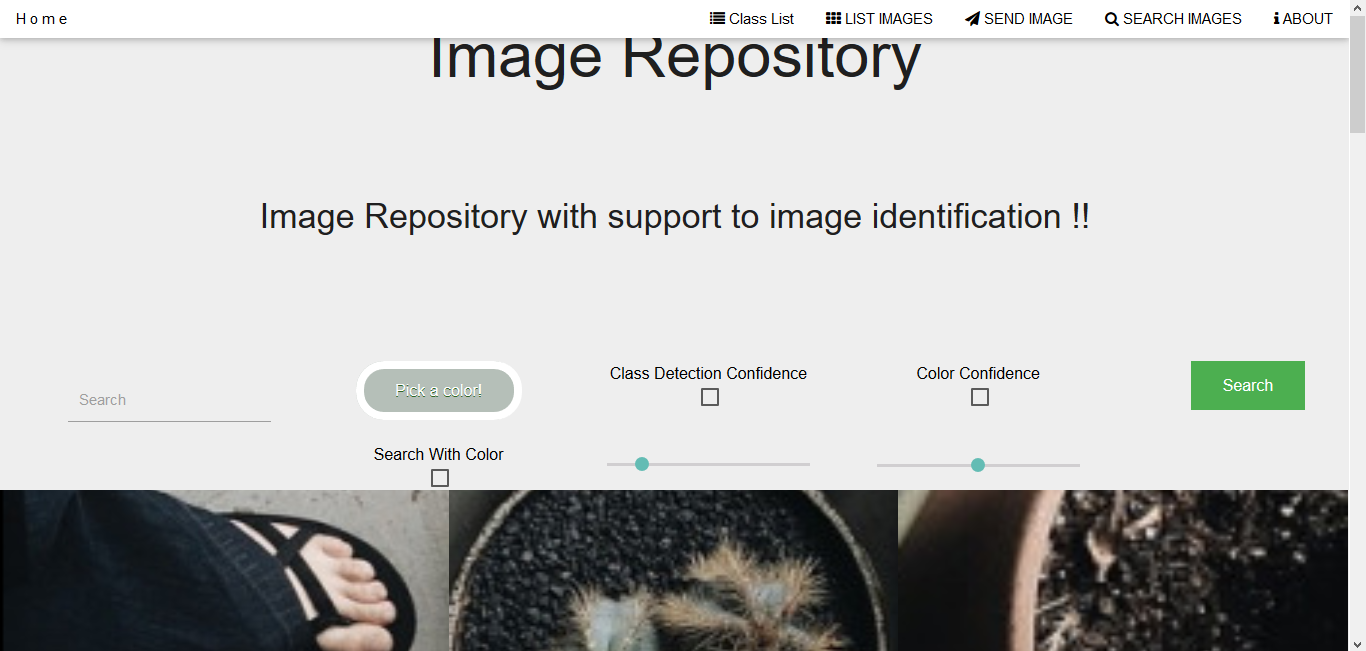
\includegraphics[width=\textwidth]{SearchDefault.png}
\caption{Página de pesquisa sem dados inseridos}
\label{Fig6}
\end{figure}

\begin{figure}[H]
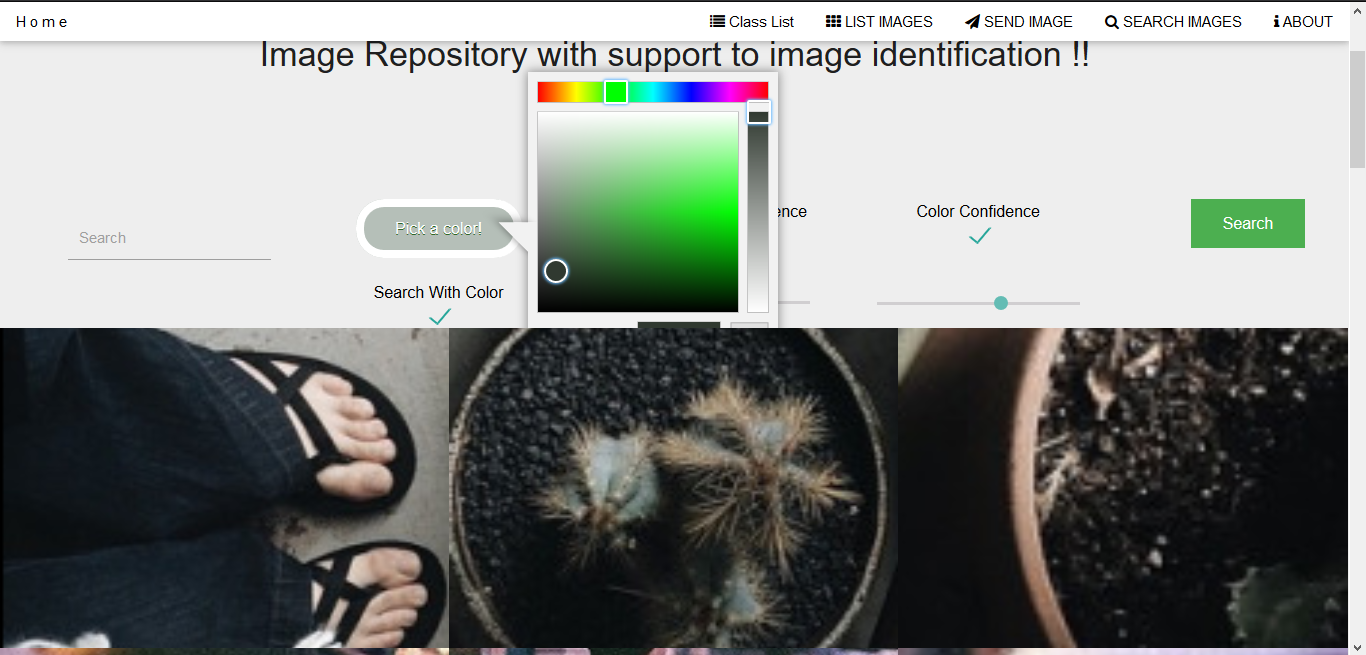
\includegraphics[width=\textwidth]{SearchWithColor.png}
\caption{Página de pesquisa por cor}
\label{Fig7}
\end{figure}

\begin{figure}[H]
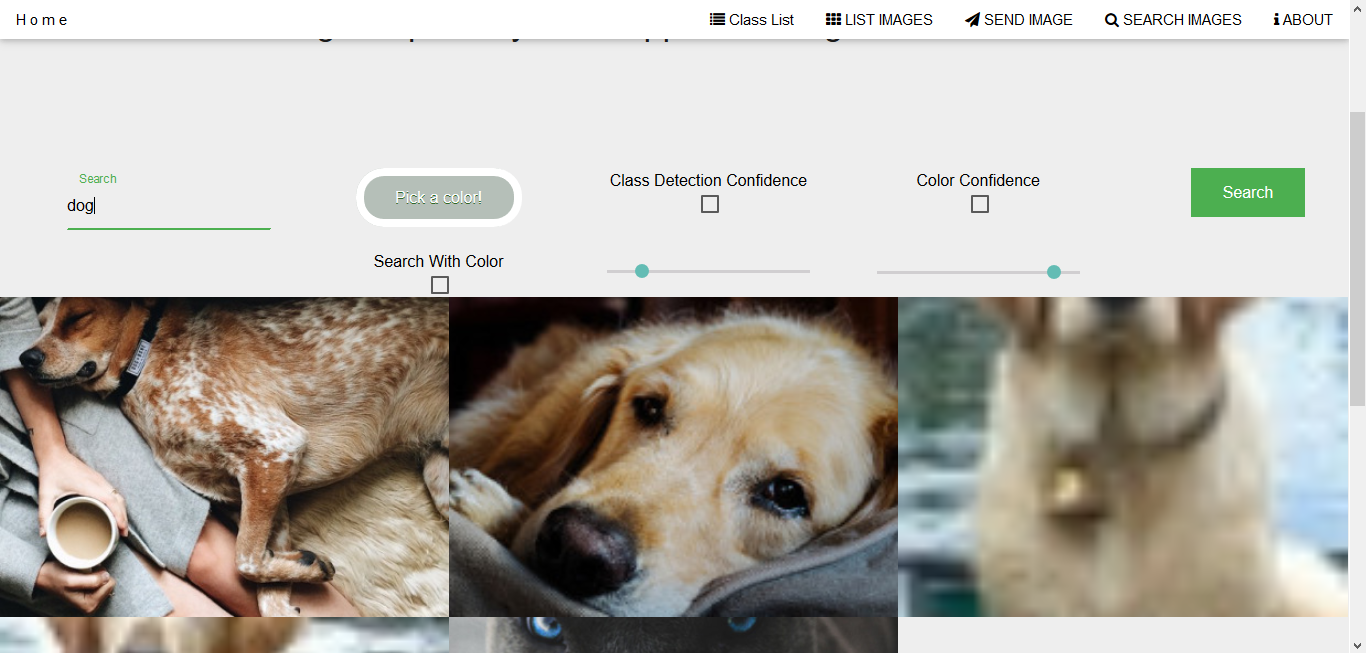
\includegraphics[width=\textwidth]{ClassSearch.png}
\caption{Página de pesquisa por classe}
\label{Fig8}
\end{figure}

Na imagem \ref{Fig9} está representada a página de sumbissão de imagens, sendo esta a página que possibilita a inserção de imagens por cada utilizador.

\begin{figure}[H]
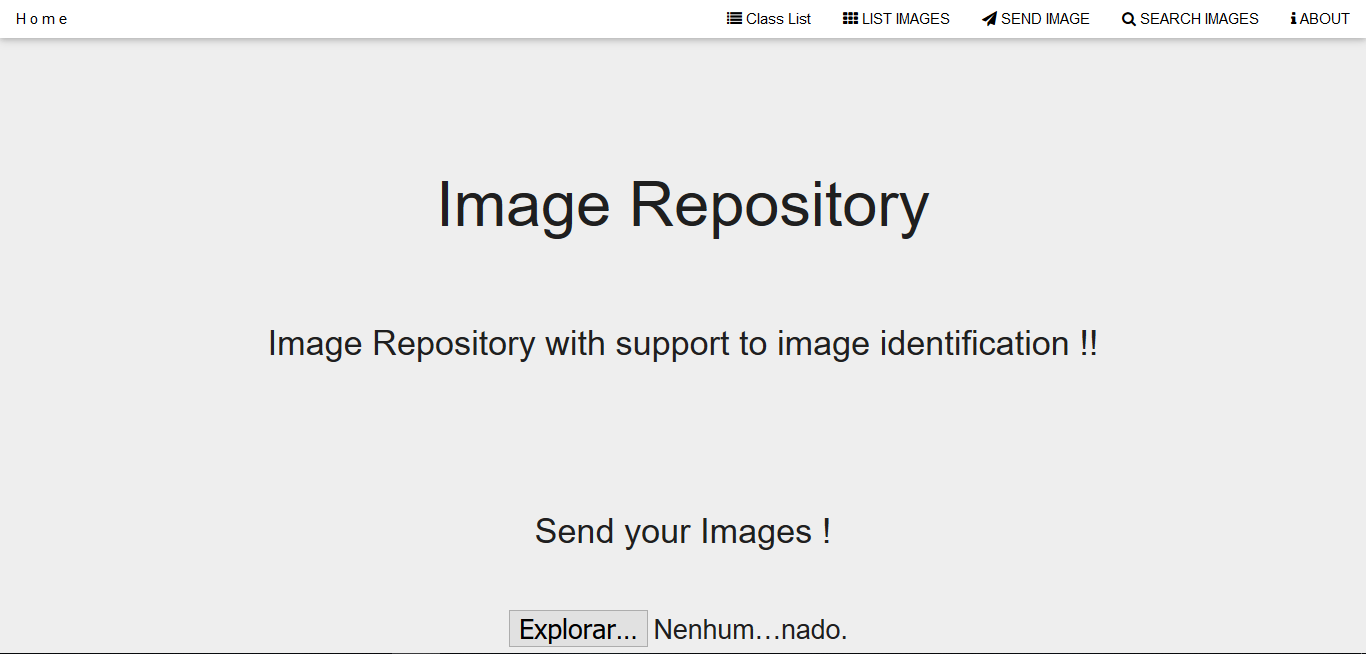
\includegraphics[width=\textwidth]{Send.png}
\caption{Página de submissão de imagens}
\label{Fig9}
\end{figure}


\chapter{Análise}
\label{chap.analise}
Segundo as figuras \ref{Fig1} e \ref{Fig2} é possível concluir que a lista de classes é feita corretamente e os exemplos de imagens também são satisfatórios.
Para além disso, na figura \ref{Fig3} é de notar que as \textit{bounding boxes} estão colocadas corretamente e a legenda de cada uma também. Por vezes há erros na classificação de classes, mas é de notar que são erros vindos do API disponibilizado pelos professores.
Cruzando os dados da figura \ref{Fig3} e \ref{Fig4} é de ver que o efeito \textit{hover} mostra os mesmos dados que a página de inspeção de imagem, portanto, os dados são congruentes.
Na figura \ref{Fig7} é possível ver a pesquisa por cor. Apesar desta ter uma implementação que nem sempre tem os dados corretos, é uma implementação satisfatória na maioria das vezes.
No que toca à pesquisa por classe (figura \ref{Fig8}) é de notar que as imagens mostradas têm, de facto, a classe correta associada  (sendo esta a classe visível na inspeção de imagens). Mais uma vez, poderá haver erros na classificação de imagens mas, mais uma vez, isso são erros vindos do API disponibilizado.
Para além disto, temos também que a submissão de imagens por utilizadores também funciona satisfatoriamente. 


\chapter{Conclusões}
\label{chap.conclusao}
O resultado final deste projeto é um \textit{website} funcional como pedido no guião. Para além disso, a utilização é extremamente intuitiiva para o utilizador e, com a compatibilidade de ecrâs é, acima de tudo, útil. Com isto, podemos dizer que o projeto foi bem suceiddo.

\chapter*{Contribuições dos autores}
A componente \textit{backend} foi feita por \ac{AP}. O\textit{frontend} foi feito por \ac{AP} e \ac{GT}. O relatório foi escrito por \ac{SV} e revisto por \ac{AP}.
As contribuições percentuais são visíveis na tabela \ref{tab2}.
\begin{table}[h!]
\begin{center}
\caption{Contribuições percentuais por aluno}
\begin{tabular}{l|l}
\hline
\multicolumn{1}{|l|}{Aluno} & \multicolumn{1}{l|}{Contribuição percentual} \\ \hline
            \ac{AP}   & 50\%                               \\ 
            \ac{GT}     & 25\%                               \\
            \ac{SV}         & 25\%                                
\end{tabular}
\label{tab2}
\end{center}
\end{table}


%%%%%%%%%%%%%%%%%%%%%%%%%%%%%%%%%
\chapter*{Acrónimos}
\begin{acronym}
\acro{ua}[UA]{Universidade de Aveiro}
\acro{miect}[MIECT]{Mestrado Integrado em Engenharia de Computadores e Telemática}
\acro{lei}[LEI]{Licenciatura em Engenharia Informática}
\acro{glisc}[GLISC]{Grey Literature International Steering Committee}
\acro{HTML}[HTML]{HyperText Markup Language}
\acro{JS}[JS]{JavaScript}
\acro{CSS}[CSS]{Cascading Style Sheets}
\acro{json}[JSON]{JavaScript Object Notation}
\acro{AP}[AP]{André Patacas}
\acro{GT}[GT]{Gil Teixeira}
\acro{SV}[SV]{Sofia Vaz}
\end{acronym}


%%%%%%%%%%%%%%%%%%%%%%%%%%%%%%%%%
\printbibliography

\end{document}
